
\section{Introduction}
    \subsection{QCD}
    \label{Intro:QCD}
        The fundamental components of the matter around us are elementary particles. The behaviour of elementary particles, such as quarks and gluons, is described by quantum field theory. In particular, quarks and gluons possess degrees of freedom called color, the physics governing this degree of freedom is known as Quantum Chromodynamics (QCD).\@ QCD is based on an SU(3) gauge theory and describes the strong interaction. The QCD Lagrangian is expressed as follows:
        \begin{eqnarray}
            \label{QCDlagrangian}
            \mathcal{L}_{QCD}=\sum_q \bar{\psi}_{q,a}\qty(i\gamma^\mu\partial_\mu-m_q)\psi_{q,a}+g_s \sum_q \bar{\psi}_{q,a}\gamma^\mu T^A_{ab}\psi_{q,b}G^A_\mu-\frac{1}{4}G^A_{\mu\nu}G^{A\mu\nu}
        \end{eqnarray}
        $\psi_{q,a}$ and $\bar{\psi}_{q,a}$ represent the quark and antiquark fields, where $q$ denotes the flavor degree of freedom, and $a$ denotes the color degree of freedom. $\gamma^\mu$ is the gamma matrics, $m_q$ is the quark mass corresponding to each flavor, $g_s$ is the QCD coupling constant, $T^A_{ab}$ are the generator matrices, $G^A_\mu$ is the gluon field, and $G^A_{\mu\nu}$ is the gluon field tensor.

        The first term in (\ref{QCDlagrangian}) represents the term for a free particle of mass $m$, the second term represents the interaction between quarks and gluons, and the third term represents the interaction between gluons themselves. A significant difference from Quantum Electrodynamics (QED), which describes electromagnetic interactions, is the presence of the coupling constant $\alpha_s(Q^2)$ and the self-interaction of the gluon field. In QED, the coupling constant does not depend on the energy scale. However, the coupling constant $\alpha_s(Q^2)$ that appears in QCD depends on the energy scale.
        \begin{figure}[htbp]
            \centering
            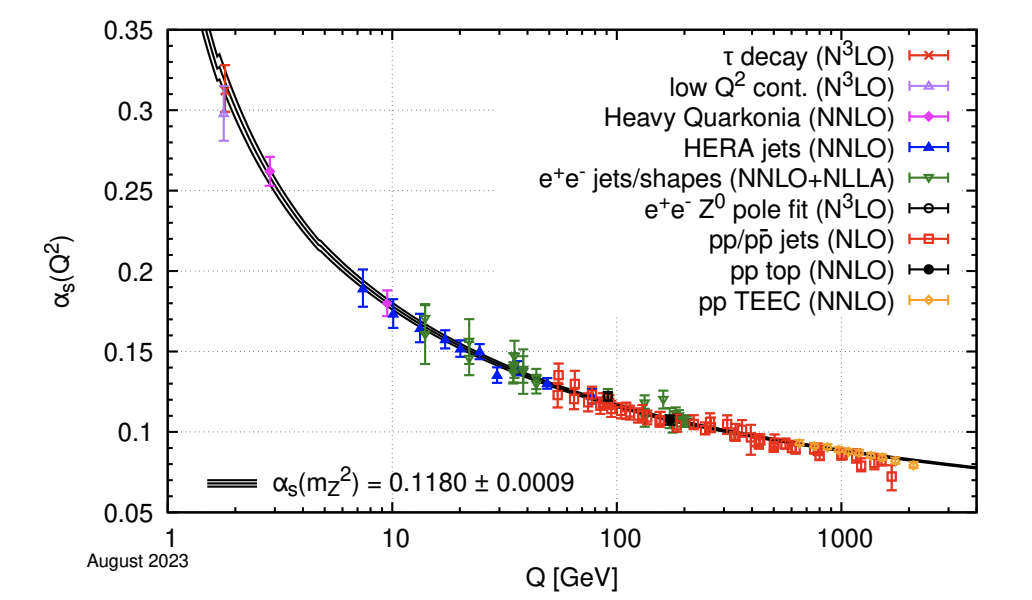
\includegraphics[keepaspectratio, scale=0.6]{fig/1_1_coupling_constant.png}
            \caption{$Q^2$ dependence of QCD coupling constants}
            \label{coupling_constant}
        \end{figure}
        Figure \ref{coupling_constant} shows how the coupling constant $\alpha_s(Q^2)$ changes with the energy scale\cite{ParticleDataGroup:2024cfk}. The coupling constant becomes small at high energy scales, corresponding to short distances. This reflects the phenomenon of asymptotic freedom, where quarks behave as free particles when they are sufficiently close to each other. On the other hand, at low energy scales corresponding to long distances, the coupling constant grows infinitely large. This represents the phenomenon of quark confinement, where quarks cannot be isolated as individual particles.
        
        Next, we focus on gluon selfinteraction. The gluon field tensor is expressed as:
        \begin{eqnarray}
        \label{eq01}
            G^A_{\mu\nu} = \partial_\mu G^A_\nu - \partial_\nu G^A_\mu + g_s f^{ABC}G^B_\mu G^C_\nu
        \end{eqnarray}  
        where $f^{ABC}$ are the structure constants of the SU(3) group. Substituting this into the third term of (\ref{QCDlagrangian}), we obtain:  
        \begin{eqnarray}
            \nonumber
            -\frac{1}{4}G^A_{\mu\nu} G^{A\mu\nu} &=& -\frac{1}{4}(\partial_\mu G^A_\nu - \partial_\nu G^A_\mu + g_s f^{ABC} G^B_\mu G^C_\nu)(\partial^\mu G^{A\nu} - \partial^{\nu} G^{A\mu} + g_s f^{ABC} G^{B\mu} G^{C\nu})\\ 
            \nonumber
            &=& -\frac{1}{4}(\partial_\mu G^A_\nu - \partial_\nu G^A_\mu)(\partial^\mu G^{A\nu} - \partial^{\nu} G^{A\mu}) \\
            \label{selfinteraction}
            && \qquad\qquad\ - g_s f^{ABC}G^B_\mu G^C_\nu \partial^\mu G^{A\nu} - g_s^2 f^{ABE}f^{CDE}G^A_\mu G^B_\nu G^{C\mu}G^{D\nu}
        \end{eqnarray}  
        %ここまで確認した%
        In (\ref{selfinteraction}), the first term represents the free gluon field without interactions. The second term represents interactions involving three gluon fields, representing reactions such as $g+g \rightarrow g$. The third term corresponds to interactions involving four gluon fields, representing reactions such as $g+g \rightarrow g+g$. For photons, the third term in \eqref{eq01} does not exist, so the second and third terms in (\ref{selfinteraction}) do not appear. This is because gluons interact with each other due to their color degrees of freedom, which gives rise to gluon selfinteraction.

        These characteristics—namely, the coupling constant's energy dependence and the gluons' selfinteraction—contribute to the complex structure of the quark-gluon interactions.
    \subsection{Chiral symmetry}
    \label{Intro:Chiral_symmetry}  
        The quark field can be separated into its right-handed and left-handed components. The projection operators for the right-handed and left-handed components are defined as $P_R$ and $P_L$, respectively. Using the $\gamma_5 = i \gamma_0 \gamma_1 \gamma_2 \gamma_3 $ matrices, they are expressed as follows:    
        \begin{eqnarray}
            P_R = \frac{1+\gamma_5}{2}, \quad P_L = \frac{1-\gamma_5}{2}
            \label{projection_operations}
        \end{eqnarray}
        (\ref{projection_operations}) hold for these projection operators.
        \begin{equation}
            P_R + P_L = 1, \quad P_R P_L = 0, \quad P_R^2 = P_R, \quad P_L^2 = P_L  
        \end{equation}
        The right-handed quark field $q_R$ and the left-handed quark field $q_L$ are expressed using the projection operators as follows:  
        \begin{eqnarray}  
            q_R = P_R q, \quad q_L = P_L q
        \end{eqnarray}  
        These components are applied to the QCD Lagrangian:  
        \begin{eqnarray}  
            \mathcal{L}_{QCD} = \sum_q \bar{q}\qty(i\gamma^\mu D_\mu - m)q
        \end{eqnarray}  
        
        \begin{itemize}
            \item Kinetic Term (First Term of the QCD Lagrangian)
                    \begin{eqnarray}  
                        \bar{q}\qty(i\gamma^\mu D_\mu)q &=& \bar{q}\qty(i\gamma^\mu D_\mu)\qty(P_R^2 + P_L^2)q \\  
                        &=& \bar{q} P_L \qty(i\gamma^\mu D_\mu) P_R q + \bar{q} P_R \qty(i\gamma^\mu D_\mu) P_L q \\  
                        &=& \bar{q}_R \qty(i\gamma^\mu D_\mu) q_R + \bar{q}_L \qty(i\gamma^\mu D_\mu) q_L  
                    \end{eqnarray}  
            
            \item Mass Term (Second Term of the QCD Lagrangian)
                    \begin{eqnarray}  
                        \bar{q}m q &=& \bar{q} m \qty(P_R^2 + P_L^2)q \\  
                        &=& \bar{q} P_R m P_R q + \bar{q} P_L m P_L q \\  
                        &=& \bar{q}_L m q_R + \bar{q}_R m q_L
                    \end{eqnarray}  
        \end{itemize}
        
        From the above, the kinetic term of the quark field can be separated into the right-handed and left-handed quark fields, thereby preserving chiral symmetry. However, the mass term mixes the right-handed and left-handed quark fields, breaking chiral symmetry. Considering the chiral limit ($m_q = 0$), the QCD Lagrangian preserves chiral symmetry.  
        
        The quark represents the order parameter for the spontaneous breaking of chiral symmetry condensate $< \bar{q}q >$. As shown in Figure \ref{quark_condensate}\cite{Weise:1993ax}, this quantity takes a finite value in the ground state of hadrons at standard temperature and density. But, it is expected to approach $< \bar{q}q > \sim 0$ at extremely high temperatures and densities. 
        \begin{figure}[htbp]  
            \centering  
            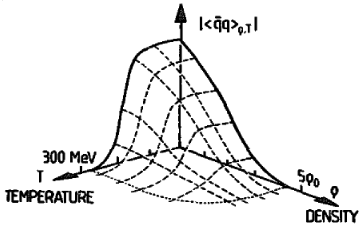
\includegraphics[keepaspectratio, scale=0.6]{fig/1_1_quark_condensate.png}  
            \caption{Temperature and density dependence of the expected value of quark condensation}  
            \label{quark_condensate}  
        \end{figure}  
        
        Since the vacuum expectation value of the quark condensate cannot be directly measured, as described later, various other probes are used to investigate the restoration of chiral symmetry.
    \subsection{NJL model}
    \label{NJL model}      
        The interaction between quarks and gluons, as described in \ref{Intro:QCD}, exhibits a complex structure, making it difficult to understand various phenomena from first-principle calculations. Therefore, models are employed to describe various phenomena. One such model is the Nambu-Jona-Lasinio (NJL), an chiral effective model. Its Lagrangian is expressed as follows.
        \begin{eqnarray}
            \label{NJLmodel}
            \mathcal{L}=\bar{q}i\gamma \cdot \partial q -(-g)\qty[(\bar{q}q)^2+(\bar{q}i\gamma_5q)^2]
        \end{eqnarray}  
        where, $q$ and $\bar{q}$ represent quark and antiquark fields, respectively; $\gamma$ and $\gamma_5$ are gamma matrices, with $\gamma_5 = i \gamma_0 \gamma_1 \gamma_2 \gamma_3$. Since there is an attractive force between quarks and antiquarks, the coupling constant $g$ is positive and has a dimension of $[\text{mass}]^{-2}$.  
        This model is an effective chiral theory for QCD at the energy scale of 1 GeV.\@ To determine the ground state of this Lagrangian, the self-consistent mean field approximation (MFA) is employed: 
        \begin{eqnarray}
            \label{sigma_ev}
            \ev{\bar{q}q}\equiv \frac{-m_0^2 \sigma}{G}\\
            \label{pi_ev}
            \ev{\bar{q}i\gamma_5q}\equiv \frac{-m_0^2 \pi}{G}
        \end{eqnarray}
        By substituting \eqref{sigma_ev} and \eqref{pi_ev} into \eqref{NJLmodel}, the expression is reformulated. Defining $\sigma = \bar{q}q$, $\pi = \bar{q} i \gamma_5 q$, and $2g = (G/m_0)^2$, we get:  
        \begin{eqnarray}
            \label{heikinbago}
            \mathcal{L}_{MFA} = \bar{q}\qty[i \gamma \cdot \partial - G(\sigma + i \pi \gamma_5)]q-\frac{m_0^2}{2}\qty(\sigma^2+\pi^2)
        \end{eqnarray}
        where, defining $q_\theta = e^{i \gamma_5 \frac{\theta}{2}} q$, $G \sqrt{\sigma^2 + \pi^2} = M$, and $\pi / \sigma = \tan{\theta}$, the Hamiltonian can be expressed as follows. $\theta$ is the parameter of the chiral transformation.  
        \begin{eqnarray}
            \label{ham}
            H_{MFA}=\int \dd[3]{\bm{x}}\qty{\bar{q}_\theta (x)(-i\gamma \cdot \nabla+M)q_{\theta}(x)+\frac{m_0^2}{2}\sigma_0^2}
        \end{eqnarray}
        where $\sigma_0^2 = \sigma^2 + \pi^2$. Since $\pi$ is considered sufficiently small, we write $\sigma$ to $\sigma_0$.  
        From this Hamiltonian, the Dirac equation for mass $M$ can be derived. Its solution is given as \ref{Msol}  
        \begin{eqnarray}
            \label{Msol}
            q_\theta (x)=\frac{1}{\sqrt{V}}\sum_{\bm{p},r=\pm} \sqrt{\frac{M}{E_p}}\qty{a_M(\bm{p},r)u_M(\bm{p},r)e^{-ip\cdot x}+b_M^{\dag}(\bm{p},r)v_M(\bm{p},r)e^{ip\cdot x}}
        \end{eqnarray}
        where, $r$ represents helicity, $E_p = \sqrt{\bm{p}^2 + M^2}$, and $M = -g\ev{\bar{q}_\theta q_\theta}$.  
        Next, when $q_\theta(x)$ is expanded using spinors with zero mass, the solution is:  
        \begin{eqnarray}
            \label{0sol}
            q_\theta (x)=\frac{1}{\sqrt{V}}\sum_{\bm{p},s=R,L}\qty{a_{\bm{p}}^{(s)}(t)u_0(\bm{p},s)e^{-i\bm{p}\cdot \bm{x}}+b_{\bm{p}}^{(s)\dag}(t)v_0(\bm{p},s)e^{i\bm{p}\cdot \bm{x}}}
        \end{eqnarray}
        where $s$ represents helicity.  
        Using the solutions (\ref{Msol}) and (\ref{0sol}), the Hamiltonian (\ref{ham}) can be expressed in terms of operators for massive and massless states. Here, $a_{\bm{p}}$ and $b_{\bm{p}}$ are expansion coefficients:  
        \begin{align}
            \label{hamenzan}
            H_{MFA} &= \sum_{\textbf{\textit{p}},s} 
            \qty{|\textbf{\textit{p}}| 
            \qty(a_{\textbf{\textit{p}}}^{(s)\dag}(t) a_{\textbf{\textit{p}}}^{(s)}(t) 
            - b_{-\textbf{\textit{p}}}^{(s)}(t)b_{-\textbf{\textit{p}}}^{(s)\dag}(t))} \notag \\
            &\hspace{5em} + M \qty(b_{-\textbf{\textit{p}}}^{(s)}(t)a_{\textbf{\textit{p}}}^{(s)}(t) 
            + a_{\textbf{\textit{p}}}^{(s)\dag}(t) b_{-\textbf{\textit{p}}}^{(s)\dag}(t)) 
            + V \frac{m_0^2}{2} \sigma_0^2 \\
            \label{massfinite}
            &= \sum_{\bm{p},r} E_p 
            \qty(a^\dagger_M(\bm{p},r)a_M(\bm{p},r) 
            - b_M(\bm{p},r)b^\dagger_M(\bm{p},r)) 
            + V \frac{m_o^2}{2} \sigma_0^2
        \end{align}
        From this Hamiltonian, the following Heisenberg equation can be derived:  
        \begin{eqnarray}
            \label{massless_Heisenberg_e.q.}
            i \mqty(\dot{a}_{\textbf{\textit{p}}}^{(s)}(t)\\\dot{b}_{-\textbf{\textit{p}}}^{(s)}(t))=\mqty(|\textbf{\textit{p}}|&M\\M&-|\textbf{\textit{p}}|)\mqty(a_{\textbf{\textit{p}}}^{(s)}(t)\\b_{-\textbf{\textit{p}}}^{(s)}(t))
        \end{eqnarray}
        Setting the initial state $a_{\bm{p}}^{(s)}(t=0) = a_{M=0}(\bm{p},s)$, the solution reveals that the massive and massless operators are connected via the Bogoliubov transformation:  
        \begin{eqnarray}
            \label{Bogoliubov transformation}
            \mqty(a_{M}(\textbf{\textit{p}},r)\\b_{M}(\textbf{\textit{p}},r)^{\dag})=U(\textbf{\textit{p}},r) \mqty(a_0(\textbf{\textit{p}},r)\\b_0(\textbf{\textit{p}},r)^{\dag})U^{\dag}(\textbf{\textit{p}},r)
        \end{eqnarray}
        where $U(\bm{p},r) = \exp{-\frac{\theta_p}{2}(a_0^\dag(\bm{p},r)b_0^\dag(-\bm{p},r) - b_0(-\bm{p},r)a_0(\bm{p},r))}$.  
        The vacuum states for each operator are defined as follows:  
        \begin{eqnarray}
            \ket{\sigma_0} &\rightarrow&a_M(\textbf{\textit{p}},r)\ket{\sigma_0}=b_M(\textbf{\textit{p}},r)\ket{\sigma_0}=0\\
            \ket{0} &\rightarrow& a_0(\textbf{\textit{p}},r)\ket{0}=b_0(\textbf{\textit{p}},r)\ket{0}=0
        \end{eqnarray}
        
       $a_0(\textbf{\textit{p}},r)^{\dag}$ creates an eigenstate of chirality, while $a_M(\textbf{\textit{p}},r)^{\dag}$ creates an eigenstate of helicity. Based on the vacuum definition and \eqref{Bogoliubov transformation}, acting on $\ket{0}$ produces an eigenstate of helicity but not a definite chirality eigenstate. This implies that "chiral symmetry is spontaneously broken".  
        
        Thus, the NJL model theoretically predicts vacuum phase transitions. In our universe, it is believed that quark condensation spontaneously breaks chiral symmetry, leading to hadrons acquiring significant masses.
    \subsection{Quark-Gluon Plasma}
        When hadrons are exposed to extremely high temperatures and densities, they transition into a plasma state known as the Quark-Gluon Plasma (QGP). In the QGP state, quarks are resolved from confinement, and chiral symmetry restoration is also expected. Furthermore, it is believed that the universe was in a QGP state immediately following the Big Bang. On the QCD phase diagram, which represents the phase structure of quarks and gluons, the QGP phase appears as shown in Figure \ref{QCD_Phase_Diagram}.    
        \begin{figure}[hbtp]
            \centering
            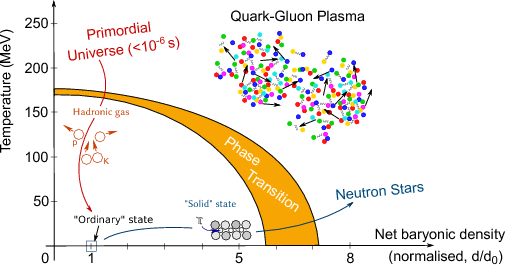
\includegraphics[keepaspectratio, scale=0.6]{fig/1_4_QCDPhaseDiagram.png}
            \caption{QCD Phase Diagram\cite{QCDPhaseDiagram}}
            \label{QCD_Phase_Diagram}
        \end{figure}
        The QGP phase can be observed in high-temperature regions in both high net baryon density and low net baryon density areas. Two types of phase transitions are related in the transition to the QGP phase. The first is the chiral phase transition. The second is the deconfinement-confinement phase transition.  
        
        The chiral phase transition is the spontaneous breaking of chiral symmetry as the vacuum undergoes a phase transition, allowing quarks to acquire a substantial effective mass. In other words, the chiral phase transition is deeply related to the mass acquisition of hadrons. 
        The deconfinement-\-confinement phase transition pertains to the con\-finement of quarks. 
        In the hadronic ground state, quarks are confined by color interaction.
        However, in the QGP state, quarks are resolved from confinement and transition into a plasma state. 
        This is the deconfinement-\-confinement phase transition. 
        While these transitions are believed to occur at approximately a similar critical temperature, this relationship is not unsolved, and research is ongoing.
        
        % Additionally, an intriguing aspect of the QCD phase diagram is the nature of phase transition orders. At zero baryon number density, lattice QCD calculations have been extensively performed, revealing that the transition is a crossover, i.e., a continuous phase transition. On the other hand, in regions with high baryon number density, lattice QCD calculations face challenges due to the sign problem, making it difficult to predict the nature of the transition. Consequently, effective models play a crucial role. Analyses based on effective models suggest that a first-order phase transition is expected. Accordingly, research exploring the locations of phase transitions on the phase diagram remains highly active.  
    \subsection{Heaby Ion collision}
        The existence of QGP, which are ultrahigh-temperature or dense materials, has been confirmed by heavy-ion collision experiments. Figure  \ref{Intro:HIC:space_time_evaluation_of_HIC} shows the time evolution proceeds in the following.
        \begin{figure}[hbtp]
            \centering
            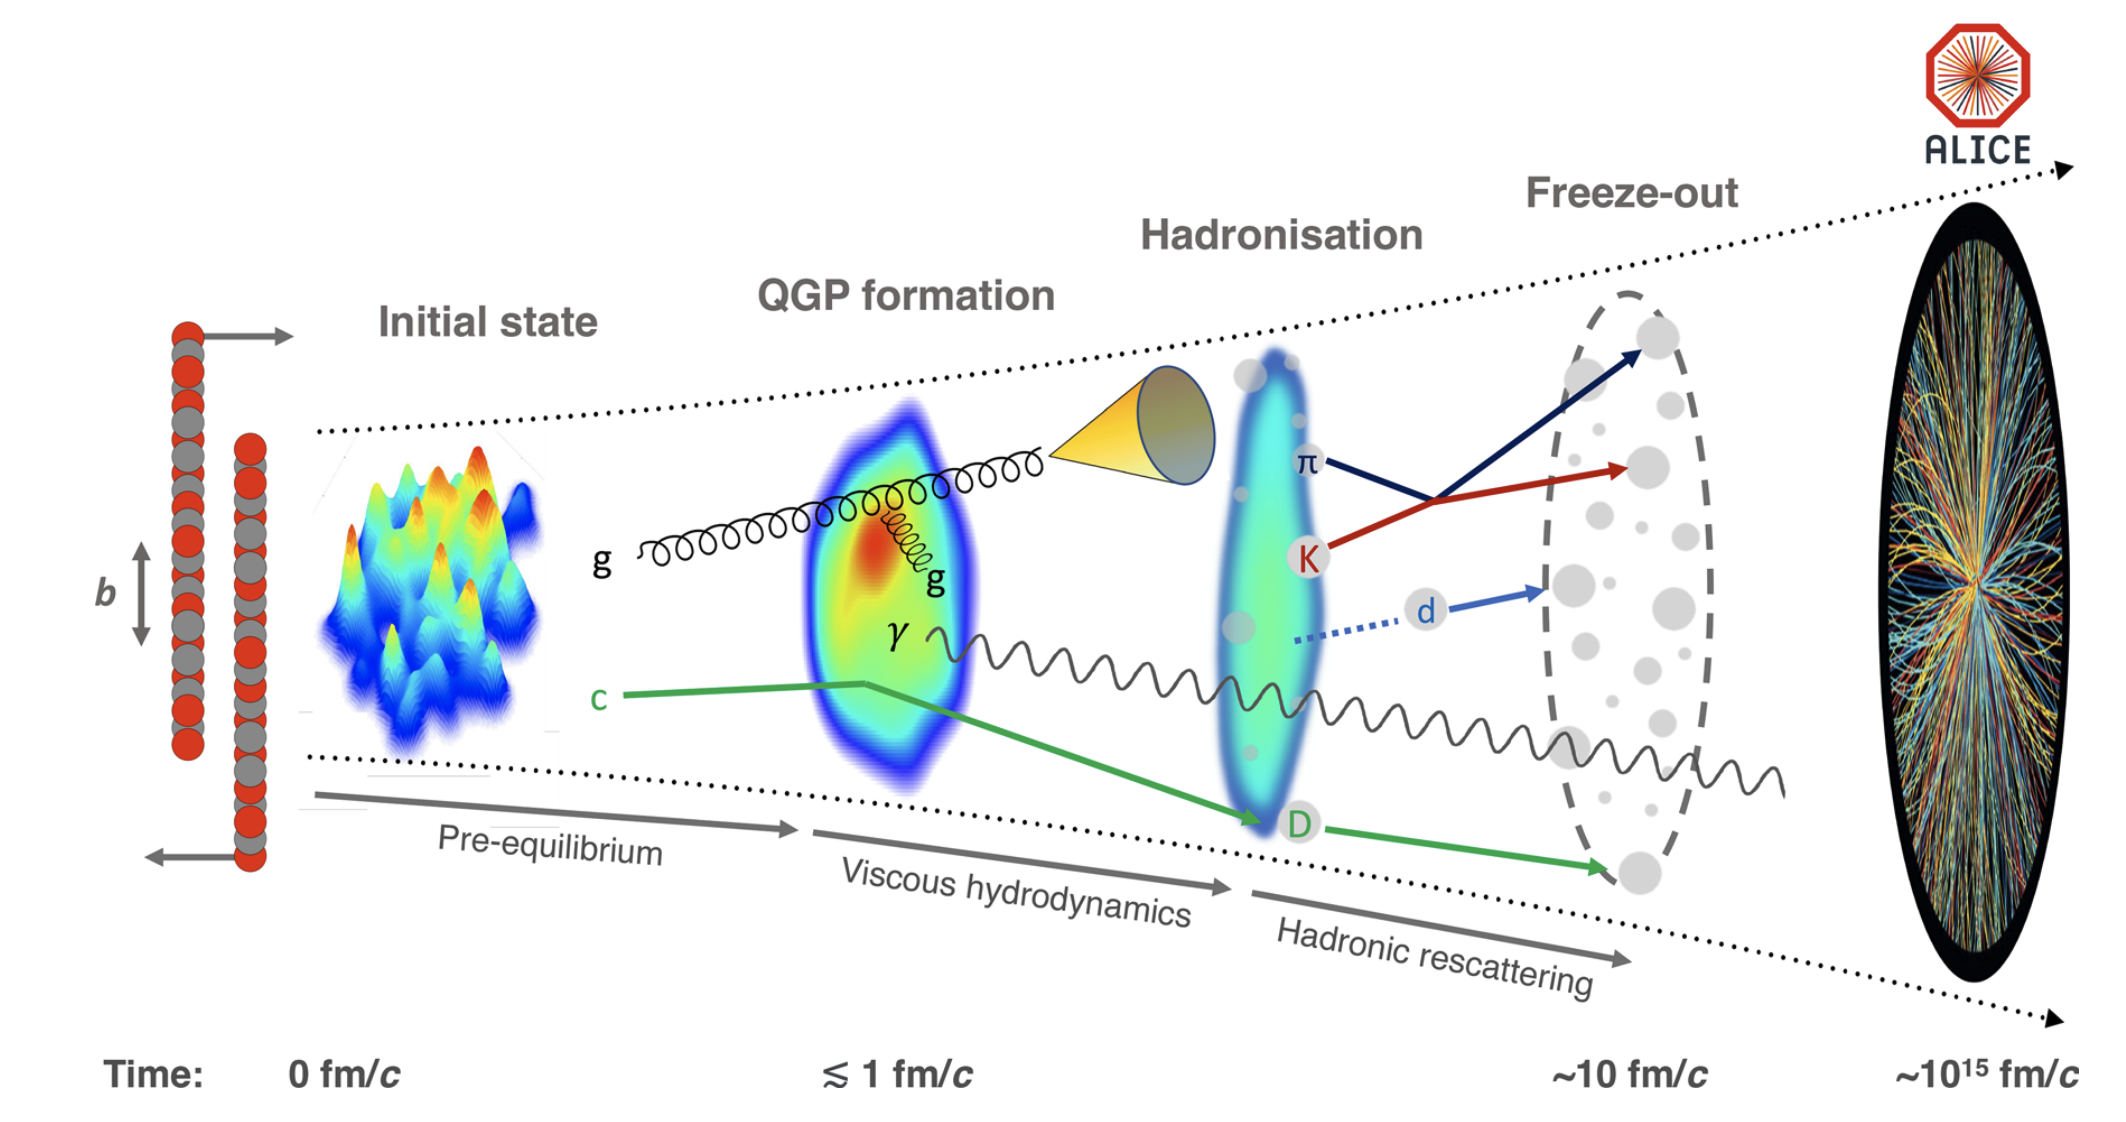
\includegraphics[keepaspectratio, scale=0.4]{fig/1_5_QGP_Evol.png}
            \caption{The evolution of a heavy-ion collision at LHC energies\cite{QGP_evo}}
            \label{Intro:HIC:space_time_evaluation_of_HIC}
        \end{figure}
        \begin{enumerate}
            \item Pre-equilibrium state
            \item QGP
            \item Hadronization
            \item Kinetic Freeze-out
        \end{enumerate}
        In the initial stage of the collision, partons from the nucleons undergo elastic and deep inelastic scatterings to reach thermalisation. During this initial collision, phenomena such as jet production and the pair production of heavy quarks occur. Once the material generated in the collision region reaches thermal equilibrium, the system transitions into the QGP state.  
        
        In the QGP state, photons and lepton pairs originating from the thermal radiation of high-temperature matter are generated. Jets interact with the QGP and lose energy, resulting in jet quenching, while heavy quarks undergo deconfinement due to the color Debye screening. Subsequently, as the QGP cools, hadronisation occurs, leading to chemical freeze-out.  
               
        Chemical freeze-out refers to stopping changes in particle species due to deeply inelastic scatterings among particles. However, elastic scatterings between hadrons continue, and momentum exchange among particles. Later, kinetic freeze-out occurs, fixing the momenta and other properties of the particles. The particles finally detected are those that remain after the kinetic freeze-out. Thus, QGP is formed during the temporal evolution of heavy-ion collisions, and its lifetime is extremely short.
        
        % Here, since partons strongly interact with the QGP, only the final state of heavy-ion collisions is observed. However, leptons and photons do not undergo strong interactions, so their measurements reflect the integration over the entire temporal evolution.
        
        % Some evidence of QGP includes jet quenching and strong elliptic flow. Jet quenching refers to the phenomenon where high-energy partons produced during the initial stage of high-energy collisions generate numerous high-momentum particles along their flight direction. However, due to their interactions with the QGP, the jets are quenched. High-energy partons passing through the medium lose energy, suppressing the jet phenomenon. Additionally, strong elliptic flow occurs when QGP generated during heavy-ion collisions exhibits a distinct collective flow depending on its density and temperature.
        The QGP generated in heavy-ion collisions has its density and temperature determined by the collision energy. High-density QGP regions are realised at collision energies of $\sqrt{s_{NN}} \lesssim 10$ [GeV].\@ At these energies, the colliding particles stop at the collision point. They create a high-density state where kinetic energy is converted directly into heat, increasing the temperature.  
  
        On the other hand, high temperature, low net baryon density regions are achieved at collision energies of $\sqrt{s_{NN}} \gtrsim 100$ [GeV].\@ In this energy regime, the colliding particles do not stop but pass through each other, producing many pair creations. As a result, the baryon number density does not become large relative to the temperature. However, a high energy density region leads to the creation of high-temperature matter near the collision point.  
               
        In the ALICE experiment, LHC Run 3 operations began in 2022, initiating Pb-Pb collision measurements at $\sqrt{s_{NN}} = 5.36$ TeV.\@ This collision energy produces QGP in the ultrahigh temperature, low net baryon density region. Moreover, compared to the QGP generated at $\sqrt{s_{NN}} = 200$ GeV at RHIC, the higher collision energy at LHC enables the measurement of a larger QGP than ever before.
    \subsection{Dilepton Measurement}
        Dilepton measurement is a good probe for investigating the time evolution of heavy-ion collisions. Leptons do not interact with strong interactions, making them less affected by the QGP.\@ This characteristic allows for the measurement of a distribution that sums up dileptons from all stages of heavy-ion collisions. The sources of dilepton production are as Figure \ref{Intro:Dilepton:dilepton_source}.
        \begin{figure}[hbtp]
            \centering
            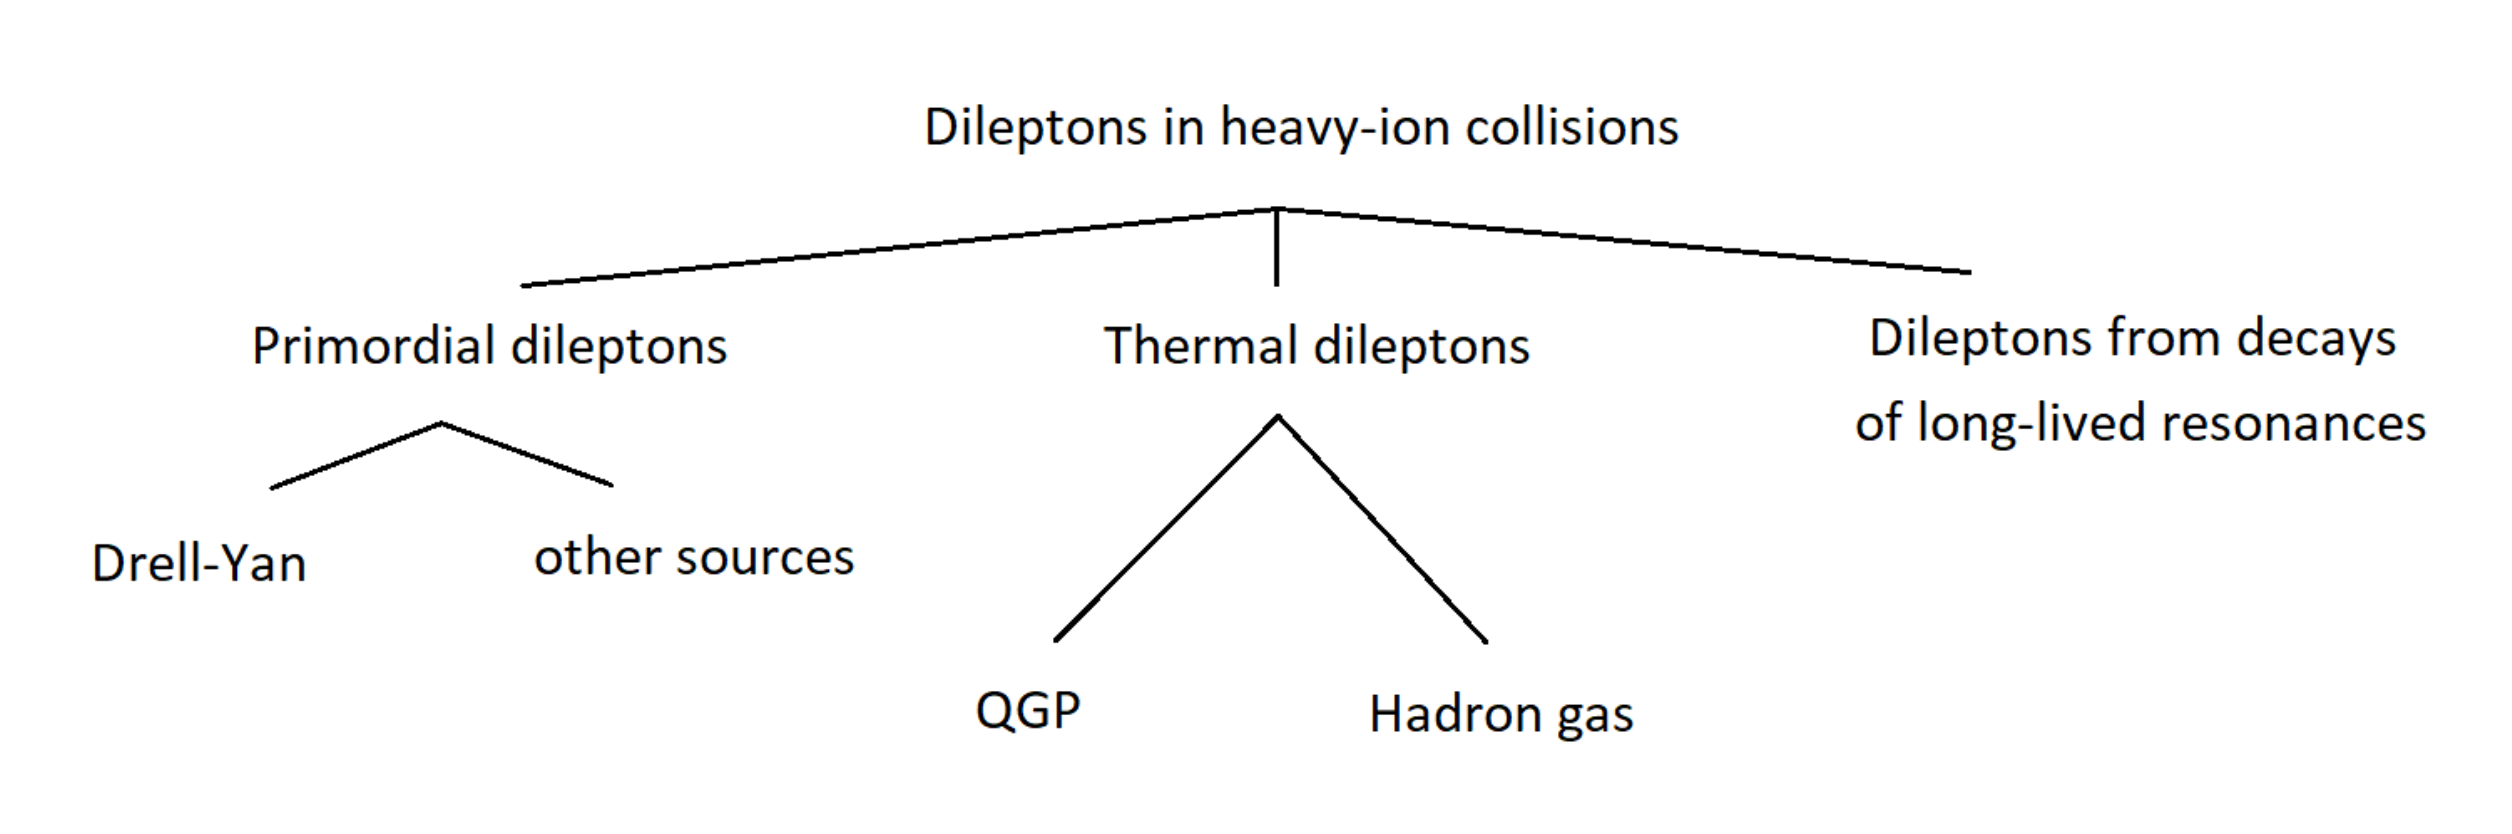
\includegraphics[keepaspectratio, scale=0.3]{fig/1_5_dilepton_source.png}
            \caption{Dilepton source\cite{Geurts:2022xmk}}
            \label{Intro:Dilepton:dilepton_source}
        \end{figure}
        
        \begin{itemize}
            \item Primordial dileptons (from \(q\bar{q}\) annihilation)
            \item Thermal dileptons
            \item Dileptons from hadron decays
        \end{itemize} 
        The dilepton mass regions are associated with the time evolution of heavy ion collisions respectively.
        \begin{figure}[hbtp]
            \centering
            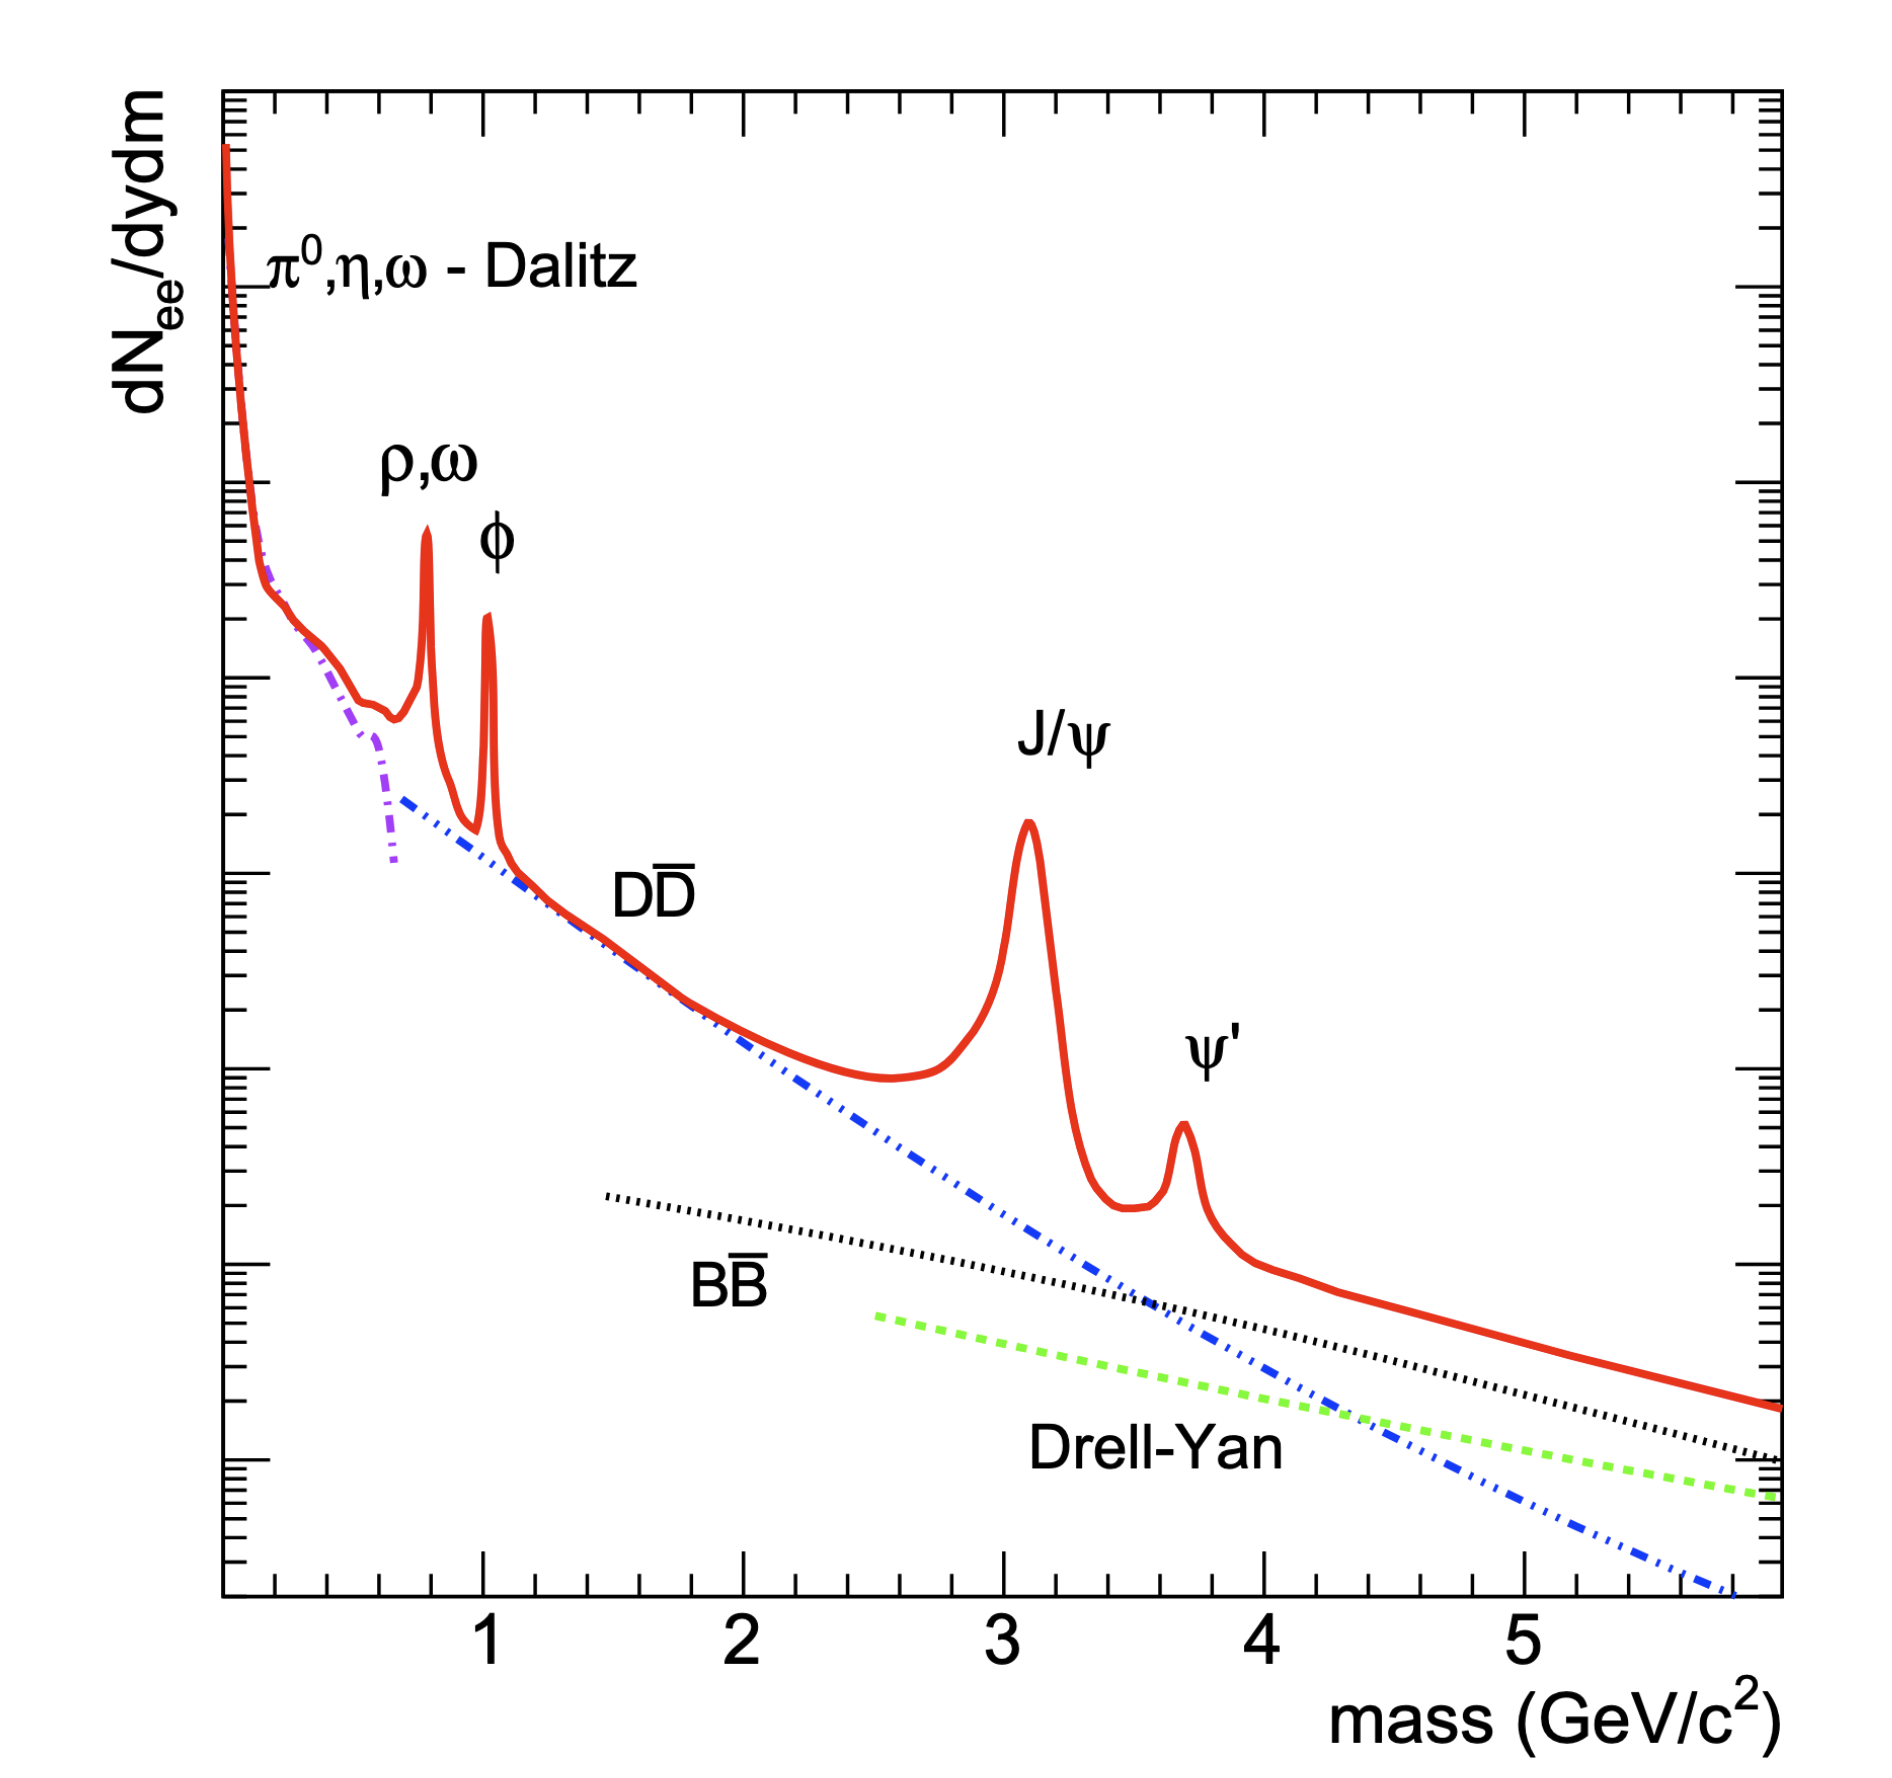
\includegraphics[keepaspectratio, scale=0.3]{fig/1_6_expected_dileptonMass.png}
            \caption{Expected mass spectrum from dileptons\cite{Rapp:1999ej}}
            \label{Intro:Dilepton:dilepton_mass}
        \end{figure}      
        In the High-Mass Region, primordial dileptons (Drell-Yan) constitute the continuum component of the mass distribution. It is related to the initial state of the collision. In the Intermediate-Mass Region, thermal dileptons originating from the QGP and continuum components such as open-charm and open-beauty are observed. 
        
        Finally, in the Low-Mass Region, the Dilepton distribution predominantly derives from light meson decays from the hadronic gas. Most dileptons from hadron decays have longer lifetimes than the QGP.\@ So these mesons observed in this region are mostly from the hadron gas. However, light vector mesons $(\rho, \omega, \phi)$ have extremely short lifetimes. The effect of the QGP has been suggested.\@
    \subsection{Search for chiral symmetry restoration in QGP}
        \begin{figure}[hbtp]
            \centering
            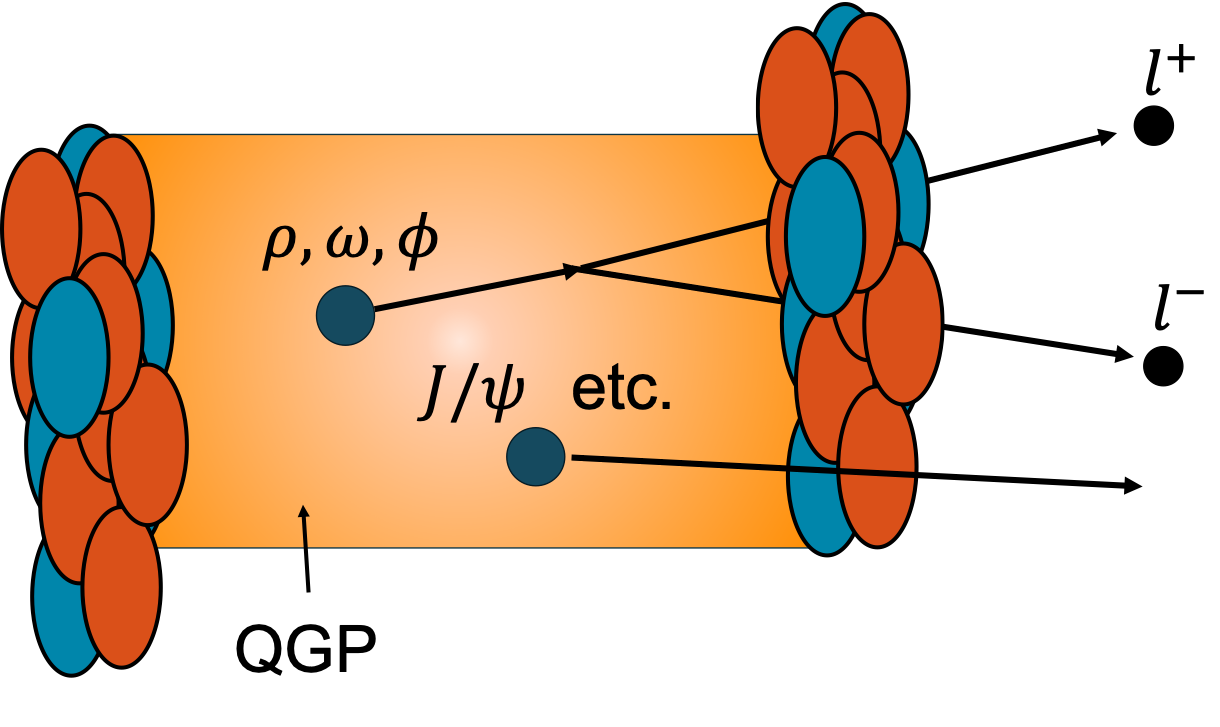
\includegraphics[keepaspectratio, scale=0.2]{fig/1_7_Search_for_chiral.png}
            \caption{Low mass vector meson decay in QGP}
            \label{Intro:Search_for_CSR:Low_mass_vector_meson_decay_in_QGP}
        \end{figure}     
        In the QGP, an ultra-high temperature and high-density state are expected to be realised, leading to $ < \bar{q}q > \sim 0 $ and restoring chiral symmetry. Light vector mesons $(\rho, \omega, \phi)$ serve as probes for the masses of hadrons in the QGP.\@ These particles have short lifetimes and decay channels into dileptons. As shown in Figure \ref{Intro:Search_for_CSR:Low_mass_vector_meson_decay_in_QGP}, their short lifetimes make it possible for them to decay within the QGP, which would otherwise immediately hadronise. Additionally, since they decay exclusively into dileptons, which do not undergo strong interactions with the QGP, the masses of hadrons within the QGP can be measured.  
        
        In past experiments, the restoration of chiral symmetry was investigated using dileptons. In the SPS-NA60 experiment, the excess of muon pairs in the low-mass region was reported. However, the excess could also be explained by $\pi + \pi \rightarrow \rho \rightarrow \pi \pi$; thus, it did not serve as definitive evidence of chiral symmetry restoration\cite{NA60}.  
        
        Additionally, in the electron pair measurements during ALICE Run 2 $\sqrt{s_{NN}} = 5.02$ TeV PbPb collisions, contributions from open-charm and open-beauty were estimated along with the vacuum dilepton distribution excluding $\rho$, and an excess of electron pairs was reported. The excess was explained as thermal dileptons from the QGP within the error range demonstrated\cite{ALICE:2023jef}. 
    \subsection{Analysis of pp collision data as a baseline}
    This paper presents the analysis results of proton-proton collision events. The particles generated in proton-proton collisions are produced from the vacuum. Measurements of collision events where QGP is not produced serve as a baseline for comparison with events where QGP is generated. The quality of track reconstruction is still insufficient, and the muon pair analysis is also incomplete. Furthermore, the quality of muon tracks in heavy-ion collisions is more challenging than in proton-proton collisions due to the large number of particles generated in each event.  

    The purpose of this study is to provide an analysis as a baseline for future studies of $\sqrt{s_{NN}} = 5.02$ PbPb collisions, where QGP is expected to be generated and to improve the quality of muon tracks in ALICE Run 3 $\sqrt{s_{NN}} = 13.6$ TeV pp collisions.